\documentclass[a4paper, 12 pt, conference]{ieeeconf}  % 
\IEEEoverridecommandlockouts                              % This command is only
% needed if you want to
% use the \thanks command

\overrideIEEEmargins
% See the \addtolength command later in the file to balance the column lengths
% on the last page of the document

% Pacote de acentuação
\usepackage[brazil]{babel}
\usepackage[utf8]{inputenc}

% The following packages can be found on http:\\www.ctan.org
\usepackage{graphics} % for pdf, bitmapped graphics files
\usepackage{epsfig} % for postscript graphics files
%\usepackage{mathptmx} % assumes new font selection scheme installed
%\usepackage{mathptmx} % assumes new font selection scheme installed
\usepackage{amsmath} % assumes amsmath package installed
\usepackage{amssymb}  % assumes amsmath package installed

\usepackage[]{todonotes} % adicionar parâmetro [disable] para ocultar os comentários
\usepackage{xspace} % usado nos comentários
\usepackage[normalem]{ulem}

\newcounter{todocounter}
\setlength{\marginparwidth}{2cm}
\reversemarginpar
\newcommand{\nota}[1]{\xspace\stepcounter{todocounter}\todo[fancyline]{\thetodocounter: #1}}
\newcommand{\notain}[2]{\stepcounter{todocounter}\todo[inline]{\thetodocounter: (#1) #2}}

\title{\LARGE \bf
Relatório das práticas de aprendizado de máquina.
}

\author{Marcus V. S. Maziero$^{1}$, Paulo R. K. Nakaima$^{2}$, Vitor Hugo Borges Basseto$^{3}$% <-this % stops a space
\thanks{$^{1}$Marcus V. S. Maziero, $^{2}$Paulo R. K. Nakaima e $^{3}$Vitor Hugo Borges Basseto estão vinculados à Universidade Tecnológica Federal do Paraná, Av. Alberto Carazzai, 1640, Cornélio Procópio, Brasil. 
        {\tt\small marcus.maziero$@$outlook.com, nakaima$@$alunos.utfpr.edu.br, vitorhugobasseto$@$gmail.com}}%
}


\begin{document}


\maketitle
\thispagestyle{empty}
\pagestyle{empty}


%%%%%%%%%%%%%%%%%%%%%%%%%%%%%%%%%%%%%%%%%%%%%%%%%%%%%%%%%%%%%%%%%%%%%%%%%%%%%%%%
%%%%%%%%%%%%%%%%%%%%%%%%%%%%%%%%%%%%%%%%%%%%%%%%%%%%%%%%%%%%%%%%%%%%%%%%%%%%%%%%
\begin{abstract}
	FAZER
\end{abstract}

\begin{keywords}
	Inteligencia Artificial, Emoções, Imagens, Machine Learning.
\end{keywords}


%%%%%%%%%%%%%%%%%%%%%%%%%%%%%%%%%%%%%%%%%%%%%%%%%%%%%%%%%%%%%%%%%%%%%%%%%%%%%%%%
%
%A Tabela \ref{Tabela_Exemplo} mostra um exemplo para inserir tabelas nesse documento e a Figura \ref{Figura_Exemplo} mostra um exemplo para inserir figuras nesse documento \cite{Buerger1989}.
%
%\begin{table}[!htbp]
%    \caption{Table Type Styles}
%    \begin{center}
%        \begin{tabular}{|c|c|c|c|}
%            \hline
%            \textbf{Table}&\multicolumn{3}{|c|}{\textbf{Table Column Head}} \\
%            \cline{2-4} 
%            \textbf{Head} & \textbf{\textit{Table column subhead}}& \textbf{\textit{Subhead}}& \textbf{\textit{Subhead}} \\
%            \hline
%            copy& More table copy$^{\mathrm{a}}$& &  \\
%            \hline
%        \end{tabular}
%    \label{Tabela_Exemplo}
%    \end{center}
%\end{table}
%
%\begin{figure}[!htbp]
%    \centering
%    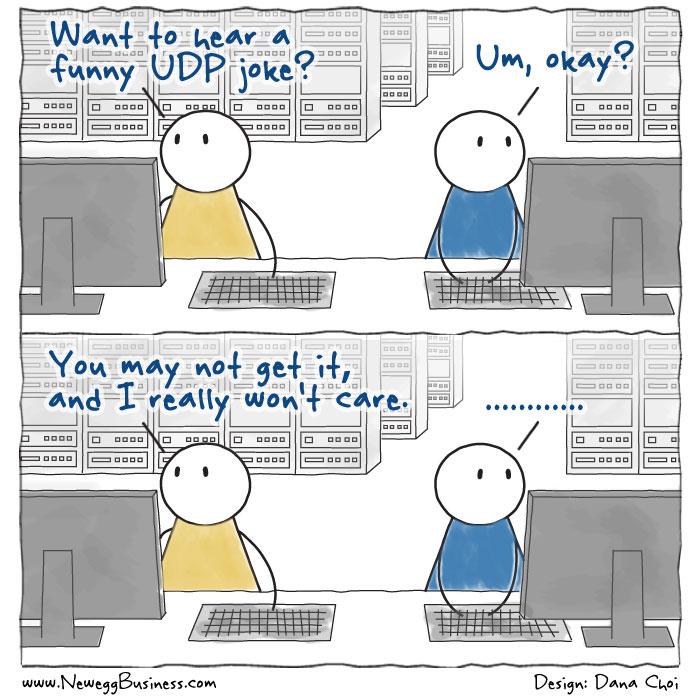
\includegraphics[width=0.8\linewidth,clip=true,trim=0cm 0cm 0cm 0cm, keepaspectratio=true]{Figura_Exemplo.png}
%    \caption{Example of a figure caption.}
%    \label{Figura_Exemplo}
%\end{figure}
%
%É importante também adicionar citações ao longo do texto para mostrar fundamentações, afirmações e trabalhos relacionados. Mais infomações sobre a adição de referências podem ser encontradas em \cite{BibTeX2014}.

\section{Prática 01}
\label{pratica01}
Nesta prática busca-se selecionar as bases de imagens e os descritores para extração de características.

\subsection{Base de dados}
Foi selecionada a base de imagens CKPLUS. A qual pode ser encontrada em: https://www.kaggle.com/shawon10/ckplus. Contém 981 imagens de rostos em escalas de cinza com as expressões de raiva, nojo, desprezo, medo, felicidade, tristeza, surpresa. Para este trabalho foram selecionadas apenas as expressões raiva, medo, felicidade, tristeza e surpresa.

A segunda base de imagens selecionada foi a Yale Face Database. A qual pode ser encontrada em: http://vision.ucsd.edu/content/yale-face-database. Contém 165 imagens em tons de cinza de rostos de 15 indivíduos fazendo 6 expressões faciais, normal, tristeza, sonolência, surpresa e piscando.

\subsection{Extração de características}
Para extração de características foi utilizado o Local Binary Patterns (LBP) e o Gabor. Sendo que o primeiro extrai 256 caracterísitcas de textura e o último 60. Os arquivos finais podem ser encontrados em: https://drive.google.com/drive/folders/1ZP-CkuoP2mQggsR2sd9QGcbks1hrt68u?usp=sharing.

\section{Prática 02}
\label{pratica02}
Nesta prática busca-se comparar diferentes classificadores com diferentes métricas a partir dos arquivos gerados na Prática \ref{pratica01}.

\subsection{Seleção da técnica de normalização}
A partir dos arquivos gerados com os descritores foram alterandas as técnicas de normalizações para verificar qual delas atinge melhor resultado para acurácia. Para a base de dados CKPLUS com o descritor LBP as diferenças são mínimas como podem ser vistas na Figura~\ref{fig:bar_norm_all}. Os classificadores utilizados foram: GaussianNB, Logistic Regression, Decision Tree K-NN, LDA, SVM, Random Forest, Neural Net.

\begin{figure}[!htbp]
	\centering
	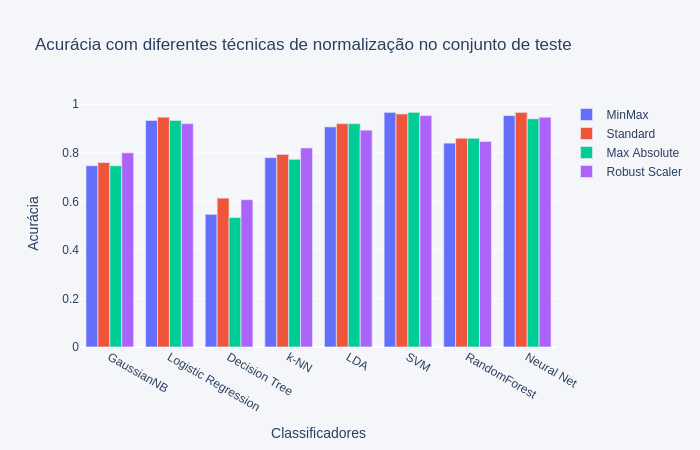
\includegraphics[width=1.0\linewidth,clip=true,trim=0cm 0cm 0cm 0cm, keepaspectratio=true]{bar_norm_all.png}
	\caption{Comparação de técnicas de normalização com descritor LBP.}
	\label{fig:bar_norm_all}
\end{figure}

Os classificadores Neural Net, SVM obtiveram os melhores resultados, 97\% de acurácia. Os piores resultados foram obtidos pelos classificadores Decision Tree 61\% e GaussianNB 80\%.

Para o descritor Gabor as diferenças entre os resultados obtidos foram altas, contudo nenhum dos classificadores obtiveram 50\% de acurácia. A técnica de normalização Min-Max que consiste em transformar cada característica com valor mínimo em 0 e os valores máximos em 1, sendo que o restando é tranformado em um valor decima entre 0 e 1, obteve a melhora acurácia. Os resultados podem ser vistos na Figura~\ref{fig:bar_norm_all_gabor} Foram mantidos os classificadores utilizados no último experimento.

\begin{figure}[!htbp]
	\centering
	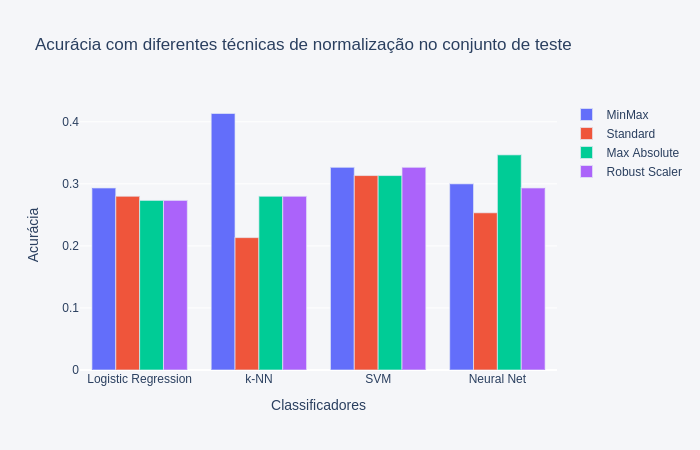
\includegraphics[width=1.0\linewidth,clip=true,trim=0cm 0cm 0cm 0cm, keepaspectratio=true]{bar_norm_all_gabor.png}
	\caption{Comparação de técnicas de normalização com descritor Gabor.}
	\label{fig:bar_norm_all_gabor}
\end{figure}


\section{Prática 03}
\label{pratica03}

Neste experimento busca-se utilizar aprendizado não supervisionado com o classificador \textit{k-means} de modo a obter o melhor valor de \textit{k}. Além disto busca-se reduzir a dimensão do conjunto de dados de modo a reter 90\% de variância.

\subsection{Redução de dimensionalidade}

Buscou-se reduzir a dimensão do conjunto de dados obtidos com o descritor LBP de modo a reter 90\% de variância. Primeiramente os dados foram normalizados com a técnica Standard, ou seja, são calculados a média e o desvio padrão da conjunto de amostras, em seguida é subraída de cada amostra a média, o resultado então é divido pelo desvio padrão. Esta técnica foi selecionada pois obteve resultado levemente superior as outras técnicas na Prática \ref{pratica02}.

Com a técnica PCA para redução de dimensionalidade foi selecionado o menor número de componentes que retinha 90\% de variância. Ver Figura~\ref{fig:points_pca_lbp}. Foi possível reduzir de 256 para 133 característica.

\begin{figure}[!htbp]
	\centering
	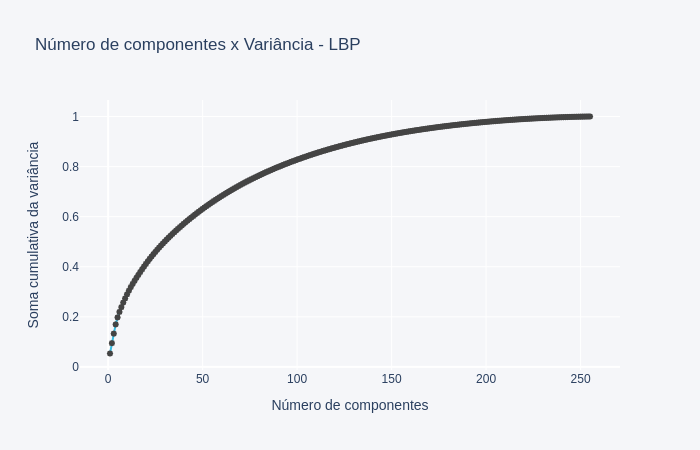
\includegraphics[width=1.0\linewidth,clip=true,trim=0cm 0cm 0cm 0cm, keepaspectratio=true]{points_pca_lbp.png}
	\caption{Selecionar o menor número de componentes retendo 90\% de variância.}
	\label{fig:points_pca_lbp}
\end{figure}

Foi aplicada a técnica PCA para as características extraídas com o descritor Gabor. Primeiramente foi normalizados os dados com a técnica MinMax, melhor resultados obtido no experimento anterior. Foi possível reduzir as características de 60 para duas retendo 100\% de variância. Ver  Figura~\ref{fig:points_pca_gabor}.

\begin{figure}[!htbp]
	\centering
	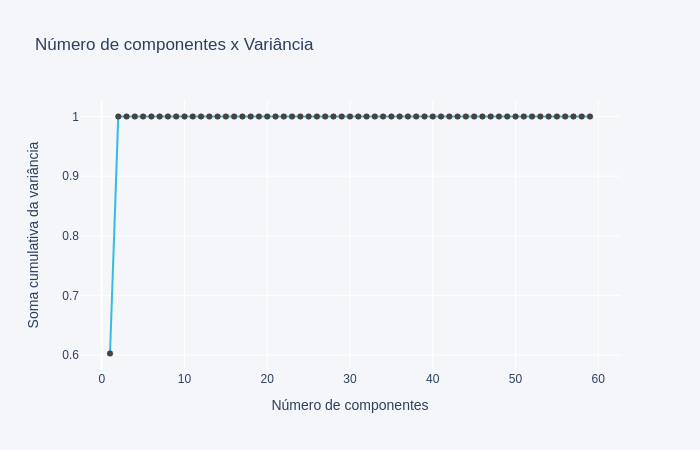
\includegraphics[width=1.0\linewidth,clip=true,trim=0cm 0cm 0cm 0cm, keepaspectratio=true]{points_pca_gabor.png}
	\caption{Selecionar o menor número de componentes retendo 100\% de variância.}
	\label{fig:points_pca_gabor}
\end{figure}


Com o conjunto de amostras reduzido foi utilizado o classificador k-means agrupando as amostras de 2 a 30 agrupamentos de forma iterativa. Ao fim, foi compilado e plotado a variância para cada quantidade de agrupamentos para aplicar-se o método elbow com intuito de definir a melhor quantidade de agrupamentos. O ponto mais distante da reta formada pela ligação do ponto inicial ao final foi 7, o melhor número de agrupamentos. Ver Figura~\ref{fig:points_elbow_lbp}. O agrupamento final foi plotado destancando-se os centróides na Figura~\ref{fig:scatter_k7_lbp}.

\begin{figure}[!htbp]
	\centering
	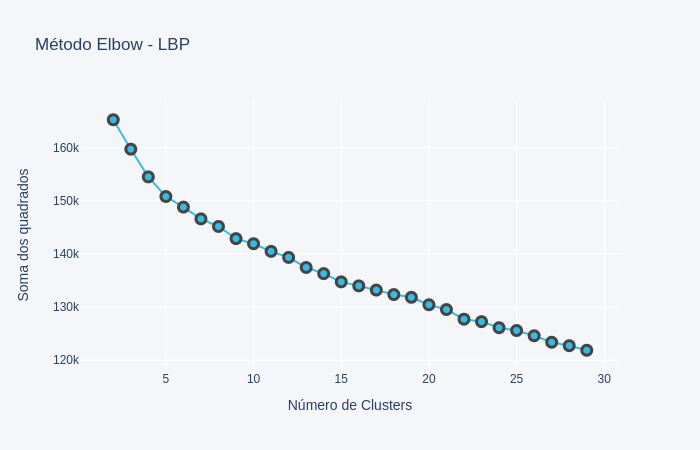
\includegraphics[width=1.0\linewidth,clip=true,trim=0cm 0cm 0cm 0cm, keepaspectratio=true]{points_elbow_lbp.png}
	\caption{Selecionar o melhor número de agrupamentos.}
	\label{fig:points_elbow_lbp}
\end{figure}

\begin{figure}[!htbp]
	\centering
	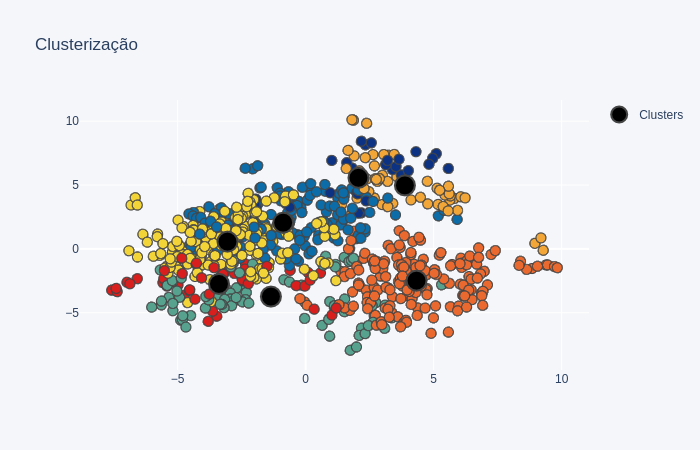
\includegraphics[width=1.0\linewidth,clip=true,trim=0cm 0cm 0cm 0cm, keepaspectratio=true]{scatter_k7_lbp.png}
	\caption{Conjuto de amostras agrupados em 7 após aplicação de PCA.}
	\label{fig:scatter_k7_lbp}
\end{figure}

\section{Prática 04}
\label{pratica04}
Nesta prática busca-se comparar os resultados de aprendizado supervisionado realizado nos experimentos anteriores com o método Label Propagation.


\subsection{Resultados}
Com relação a acurácia para o conjunto de teste utilizando o descritor LBP os resultados foram: Neural Net 97\%, SVM  95.3\%, Logistic Regression 92.6\%, LDA 91.3\%, Random Forest 90.6\%, GaussianNB  81.3\%, K-NN 78.6\%, Decision Tree 69.3\%. Estes dados podem ser vistos na Tabela ~\ref{tab:result_lbp} e Figura~\ref{fig:bar_result_lbp}.


\begin{table}[!htbp]
	\caption{Acurácia dos classificadores utilizando o descritor LBP}
	\begin{center}
		\begin{tabular}{|c|c|}
			\hline
			& Acurácia \\
			\hline
			Neural Net          & 97.3\% \\
			SVM                 & 95.3\% \\
			Logistic Regression & 92.6\% \\
			LDA                 & 91.3\% \\
			Random Forest       & 90.6\% \\
			GaussianNB          & 81.3\% \\
			K-NN                & 78.6\% \\
			Decision Tree       & 69.3\% \\
			\hline
		\end{tabular}
		\label{tab:result_lbp}
	\end{center}
\end{table}

\begin{figure}[!htbp]
	\centering
	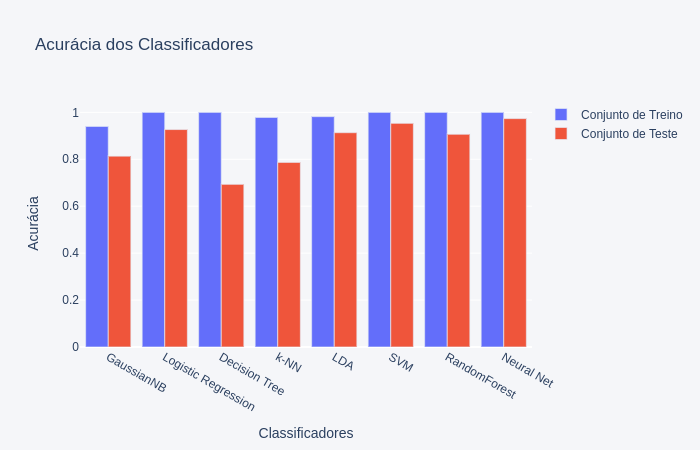
\includegraphics[width=1.0\linewidth,clip=true,trim=0cm 0cm 0cm 0cm, keepaspectratio=true]{bar_result_lbp.png}
	\caption{Acurácia para o conjunto de treino e teste com o descritor LBP}
	\label{fig:bar_result_lbp}
\end{figure}

Com o descritor Gabor os resultados foram: Random Forest 69.3\%, K-NN 62.6\%, Decision Tree 61.3\%, SVM 34\%, Neural Net 32.6\%, LDA 32\%, Logistic Regression 31.3\%, GaussianNB 27.3\%. Estes dados podem ser vistos na Tabela ~\ref{tab:result_gabor} e Figura~\ref{fig:bar_result_gabor}. Embora o desempenho dos classificadores atingirem no máximo 69.3\%, nota-se grande melhoria quando é reduzida a quantidade de características quando comparado a Figura~\ref{fig:bar_norm_all_gabor}.

\begin{table}[!htbp]
	\caption{Acurácia dos classificadores utilizando o descritor Gabor}
	\begin{center}
		\begin{tabular}{|c|c|}
			\hline
			& Acurácia \\
			\hline
			Random Forest       & 69.3\%   \\
			K-NN                & 62.6\%   \\
			Decision Tree       & 61.3\%   \\
			SVM                 & 34\%     \\
			Neural Net          & 32.6\%   \\
			LDA                 & 32\%     \\
			Logistic Regression & 31.3\%   \\
			GaussianNB          & 27.3\%   \\
			\hline
		\end{tabular}
		\label{tab:result_gabor}
	\end{center}
\end{table}

\begin{figure}[!htbp]
	\centering
	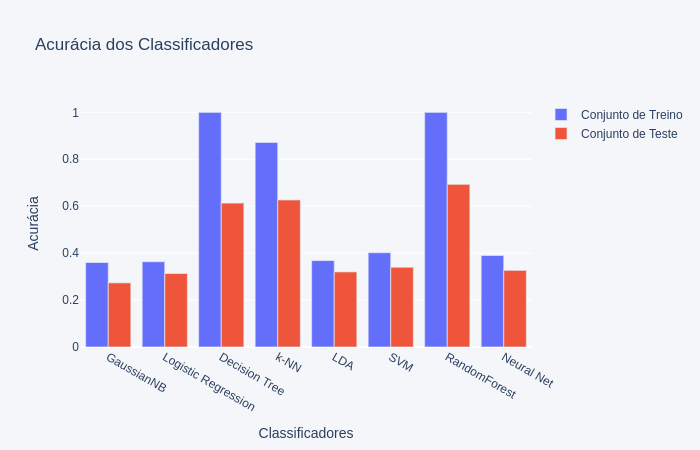
\includegraphics[width=1.0\linewidth,clip=true,trim=0cm 0cm 0cm 0cm, keepaspectratio=true]{bar_result_gabor.png}
	\caption{Acurácia para o conjunto de treino e teste com o descritor Gabor}
	\label{fig:bar_result_gabor}
\end{figure}
\section{CONCLUSÃO}

Neste trabalho foi realizado o reconhecimento de expressões faciais com aprendizado de máquina. Foram comparadas com base na acurácia o melhor desempenho para os descritores LBP e Gabor. O primeiro foi que obteve melhor resultado. Foram comparadas diferentes técnicas de normalização sendo que os testes realizados com o descritor Gabor foi o que apresentou maior sensibilidade para este tipo de alteração. Além disto foi aplicada a técnica de redução de dimensionalidade com o PCA, novamente os resultados baseados no descritor Gabor foi o mais afetado.

\bibliography{referencias}
\bibliographystyle{plain}

\end{document}
